
\chapter*{Введение}


Феномен оценки позы человека --- это проблема, которая изучалась в течение лет, в сфере компьютерного зрения. Что же это такое? Чтобы ответить на этот вопрос, необходимо понять концепцию позы. Позу можно определить как расположение суставов человека специфическим образом. Таким образом, мы можем определить проблему оценки позы человека как локализацию суставов человека или заранее определенных ориентиров на изображениях и видео. Существует несколько типов оценки позы, включая оценки тела, лица и руки (см. рисунок \ref{img:human,hand,face}), а также множество аспектов.

\begin{figure}[ht!]
	\centering
	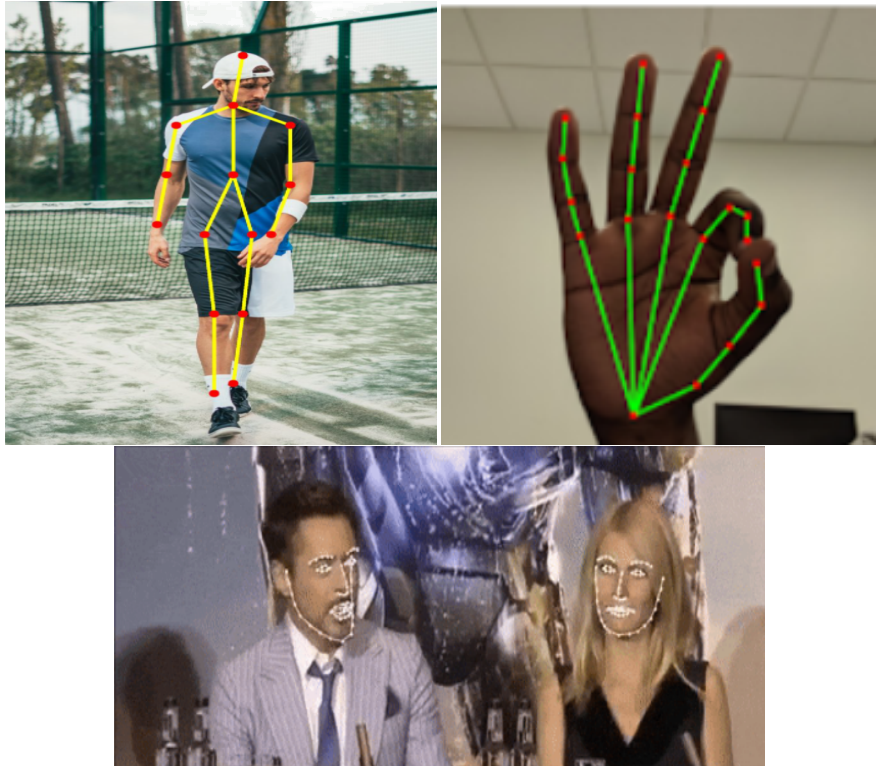
\includegraphics[width=0.96\linewidth]{assets/thefirst.png}
	\caption{Эти изображения пример разных типов определения позы человека. Верхняя левая --- это пример определения позы тела человека, верхняя правая --- это пример позы руки. Нижнее изображение --- это пример определение позы лица.}
	\label{img:human,hand,face}
\end{figure}


Целью данной работы является изучение методов определения позы человека \cite{guide-hpe}. Для достижения поставленной цели необходимо выполнить следующие задачи:
\begin{itemize}
	\item изучить методы по определению позы человека;
	\item выбрать критерии классификации и сравнить эти методы;
	\item определить области возможного применения методов определения поз человека.
\end{itemize}